%RequestPackage amsmath
% i am second line

\usetikzlibrary{calc}




\newcommand{\drawgrid}[2]{%
\draw[line cap=rect] (0,0) grid ++ (#1,#2); 
}


\newcommand{\fillcoord}[2]{%

\fill[black] (#1,#2) rectangle ++ (1,1); 

}

\newcommand{\namecoord}[4]{%

\node (#3) at ($(#1,#2)+(0.5,0.5)$) {#4}; 

}




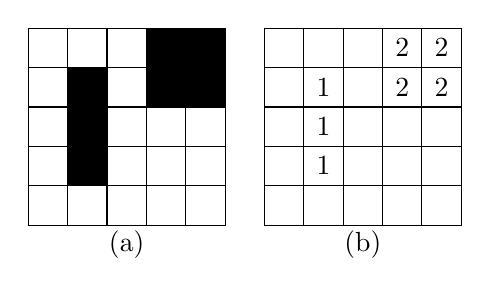
\begin{tikzpicture}[scale=0.5]


\namecoord{2}{-1}{}{(a)}




\drawgrid{5}{5}

\fillcoord{1}{1}
\fillcoord{1}{2}
\fillcoord{1}{3}


\fillcoord{3}{3}
\fillcoord{3}{4}
\fillcoord{4}{3}
\fillcoord{4}{4}


\begin{scope}[shift={(6,0)}]
\namecoord{2}{-1}{}{(b)}
\drawgrid{5}{5}

\namecoord{1}{1}{}{1}
\namecoord{1}{2}{}{1}
\namecoord{1}{3}{}{1}

\namecoord{3}{4}{}{2}
\namecoord{3}{3}{}{2}
\namecoord{4}{4}{}{2}
\namecoord{4}{3}{}{2}

\end{scope}




\end{tikzpicture}



